\documentclass[twoside]{book}

% Packages required by doxygen
\usepackage{fixltx2e}
\usepackage{calc}
\usepackage{doxygen}
\usepackage[export]{adjustbox} % also loads graphicx
\usepackage{graphicx}
\usepackage[utf8]{inputenc}
\usepackage{makeidx}
\usepackage{multicol}
\usepackage{multirow}
\PassOptionsToPackage{warn}{textcomp}
\usepackage{textcomp}
\usepackage[nointegrals]{wasysym}
\usepackage[table]{xcolor}

% Font selection
\usepackage[T1]{fontenc}
\usepackage[scaled=.90]{helvet}
\usepackage{courier}
\usepackage{amssymb}
\usepackage{sectsty}
\renewcommand{\familydefault}{\sfdefault}
\allsectionsfont{%
  \fontseries{bc}\selectfont%
  \color{darkgray}%
}
\renewcommand{\DoxyLabelFont}{%
  \fontseries{bc}\selectfont%
  \color{darkgray}%
}
\newcommand{\+}{\discretionary{\mbox{\scriptsize$\hookleftarrow$}}{}{}}

% Page & text layout
\usepackage{geometry}
\geometry{%
  a4paper,%
  top=2.5cm,%
  bottom=2.5cm,%
  left=2.5cm,%
  right=2.5cm%
}
\tolerance=750
\hfuzz=15pt
\hbadness=750
\setlength{\emergencystretch}{15pt}
\setlength{\parindent}{0cm}
\setlength{\parskip}{3ex plus 2ex minus 2ex}
\makeatletter
\renewcommand{\paragraph}{%
  \@startsection{paragraph}{4}{0ex}{-1.0ex}{1.0ex}{%
    \normalfont\normalsize\bfseries\SS@parafont%
  }%
}
\renewcommand{\subparagraph}{%
  \@startsection{subparagraph}{5}{0ex}{-1.0ex}{1.0ex}{%
    \normalfont\normalsize\bfseries\SS@subparafont%
  }%
}
\makeatother

% Headers & footers
\usepackage{fancyhdr}
\pagestyle{fancyplain}
\fancyhead[LE]{\fancyplain{}{\bfseries\thepage}}
\fancyhead[CE]{\fancyplain{}{}}
\fancyhead[RE]{\fancyplain{}{\bfseries\leftmark}}
\fancyhead[LO]{\fancyplain{}{\bfseries\rightmark}}
\fancyhead[CO]{\fancyplain{}{}}
\fancyhead[RO]{\fancyplain{}{\bfseries\thepage}}
\fancyfoot[LE]{\fancyplain{}{}}
\fancyfoot[CE]{\fancyplain{}{}}
\fancyfoot[RE]{\fancyplain{}{\bfseries\scriptsize Generated by Doxygen }}
\fancyfoot[LO]{\fancyplain{}{\bfseries\scriptsize Generated by Doxygen }}
\fancyfoot[CO]{\fancyplain{}{}}
\fancyfoot[RO]{\fancyplain{}{}}
\renewcommand{\footrulewidth}{0.4pt}
\renewcommand{\chaptermark}[1]{%
  \markboth{#1}{}%
}
\renewcommand{\sectionmark}[1]{%
  \markright{\thesection\ #1}%
}

% Indices & bibliography
\usepackage{natbib}
\usepackage[titles]{tocloft}
\setcounter{tocdepth}{3}
\setcounter{secnumdepth}{5}
\makeindex

% Hyperlinks (required, but should be loaded last)
\usepackage{ifpdf}
\ifpdf
  \usepackage[pdftex,pagebackref=true]{hyperref}
\else
  \usepackage[ps2pdf,pagebackref=true]{hyperref}
\fi
\hypersetup{%
  colorlinks=true,%
  linkcolor=blue,%
  citecolor=blue,%
  unicode%
}

% Custom commands
\newcommand{\clearemptydoublepage}{%
  \newpage{\pagestyle{empty}\cleardoublepage}%
}

\usepackage{caption}
\captionsetup{labelsep=space,justification=centering,font={bf},singlelinecheck=off,skip=4pt,position=top}

%===== C O N T E N T S =====

\begin{document}

% Titlepage & ToC
\hypersetup{pageanchor=false,
             bookmarksnumbered=true,
             pdfencoding=unicode
            }
\pagenumbering{alph}
\begin{titlepage}
\vspace*{7cm}
\begin{center}%
{\Large Frame Grabber }\\
\vspace*{1cm}
{\large Generated by Doxygen 1.8.14}\\
\end{center}
\end{titlepage}
\clearemptydoublepage
\pagenumbering{roman}
\tableofcontents
\clearemptydoublepage
\pagenumbering{arabic}
\hypersetup{pageanchor=true}

%--- Begin generated contents ---
\chapter{Hierarchical Index}
\section{Class Hierarchy}
This inheritance list is sorted roughly, but not completely, alphabetically\+:\begin{DoxyCompactList}
\item \contentsline{section}{analyze\+Imgs}{\pageref{classanalyze_imgs}}{}
\item C\+Image\+Event\+Handler\begin{DoxyCompactList}
\item \contentsline{section}{Custom\+Image\+Event\+Handler}{\pageref{class_custom_image_event_handler}}{}
\end{DoxyCompactList}
\end{DoxyCompactList}

\chapter{Class Index}
\section{Class List}
Here are the classes, structs, unions and interfaces with brief descriptions\+:\begin{DoxyCompactList}
\item\contentsline{section}{\mbox{\hyperlink{classanalyze_imgs}{analyze\+Imgs}} }{\pageref{classanalyze_imgs}}{}
\item\contentsline{section}{\mbox{\hyperlink{class_custom_image_event_handler}{Custom\+Image\+Event\+Handler}} }{\pageref{class_custom_image_event_handler}}{}
\end{DoxyCompactList}

\chapter{Class Documentation}
\hypertarget{classanalyze_imgs}{}\section{analyze\+Imgs Class Reference}
\label{classanalyze_imgs}\index{analyze\+Imgs@{analyze\+Imgs}}
\subsection*{Public Member Functions}
\begin{DoxyCompactItemize}
\item 
\mbox{\Hypertarget{classanalyze_imgs_a899a5c6c1c2f6decf3c04a373e786d2f}\label{classanalyze_imgs_a899a5c6c1c2f6decf3c04a373e786d2f}} 
void {\bfseries set\+F\+PS} (float fps)
\item 
\mbox{\Hypertarget{classanalyze_imgs_a93840314df4e33629e4454d26b23763c}\label{classanalyze_imgs_a93840314df4e33629e4454d26b23763c}} 
void {\bfseries set\+Num\+Cams} (int num)
\item 
\mbox{\Hypertarget{classanalyze_imgs_a624ba3e9d0bd3b8eafe3b805d4259a2b}\label{classanalyze_imgs_a624ba3e9d0bd3b8eafe3b805d4259a2b}} 
void {\bfseries get\+R\+OI} (cv\+::\+Mat img)
\item 
\mbox{\Hypertarget{classanalyze_imgs_a5ca9053a5848b73b448e7cc10fe0247b}\label{classanalyze_imgs_a5ca9053a5848b73b448e7cc10fe0247b}} 
cv\+::\+Mat {\bfseries binarize} (cv\+::\+Mat img)
\item 
\mbox{\Hypertarget{classanalyze_imgs_a7d731a5c365843d72fe5a1f5fffa84d0}\label{classanalyze_imgs_a7d731a5c365843d72fe5a1f5fffa84d0}} 
cv\+::\+Mat {\bfseries get\+Mask} (cv\+::\+Mat img)
\item 
\mbox{\Hypertarget{classanalyze_imgs_a79806f36d4bb2ab6beb0142464386e97}\label{classanalyze_imgs_a79806f36d4bb2ab6beb0142464386e97}} 
void {\bfseries compare\+Imgs} (cv\+::\+Mat prev\+Im, cv\+::\+Mat new\+Im)
\item 
\mbox{\Hypertarget{classanalyze_imgs_adff6d0fbf91c2c65714a817c23977fc7}\label{classanalyze_imgs_adff6d0fbf91c2c65714a817c23977fc7}} 
bool {\bfseries connect\+Analysis} (cv\+::\+Mat img, int camera)
\item 
\mbox{\Hypertarget{classanalyze_imgs_a1aa11cadf35335cf8abd7796d25a2dc4}\label{classanalyze_imgs_a1aa11cadf35335cf8abd7796d25a2dc4}} 
bool {\bfseries is\+Moving} (cv\+::\+Mat img, int camera)
\end{DoxyCompactItemize}
\subsection*{Public Attributes}
\begin{DoxyCompactItemize}
\item 
\mbox{\Hypertarget{classanalyze_imgs_ac37b6d76c04405d43ba6a6f4e6d902f8}\label{classanalyze_imgs_ac37b6d76c04405d43ba6a6f4e6d902f8}} 
cv\+::\+Mat {\bfseries image}
\end{DoxyCompactItemize}


The documentation for this class was generated from the following files\+:\begin{DoxyCompactItemize}
\item 
/\+Users/rlaporte/\+Library/\+Mobile Documents/com$\sim$apple$\sim$\+Cloud\+Docs/\+Courses/\+B\+A\+P\+R\+O\+J -\/ Neuro-\/\+Engineering Laboratory/\+Source Files/\+N\+I\+R\+\_\+\+Imaging/\+C++\+\_\+\+Source/analyze\+Imgs.\+h\item 
/\+Users/rlaporte/\+Library/\+Mobile Documents/com$\sim$apple$\sim$\+Cloud\+Docs/\+Courses/\+B\+A\+P\+R\+O\+J -\/ Neuro-\/\+Engineering Laboratory/\+Source Files/\+N\+I\+R\+\_\+\+Imaging/\+C++\+\_\+\+Source/analyze\+Imgs.\+cpp\end{DoxyCompactItemize}

\hypertarget{class_custom_image_event_handler}{}\section{Custom\+Image\+Event\+Handler Class Reference}
\label{class_custom_image_event_handler}\index{Custom\+Image\+Event\+Handler@{Custom\+Image\+Event\+Handler}}
Inheritance diagram for Custom\+Image\+Event\+Handler\+:\begin{figure}[H]
\begin{center}
\leavevmode
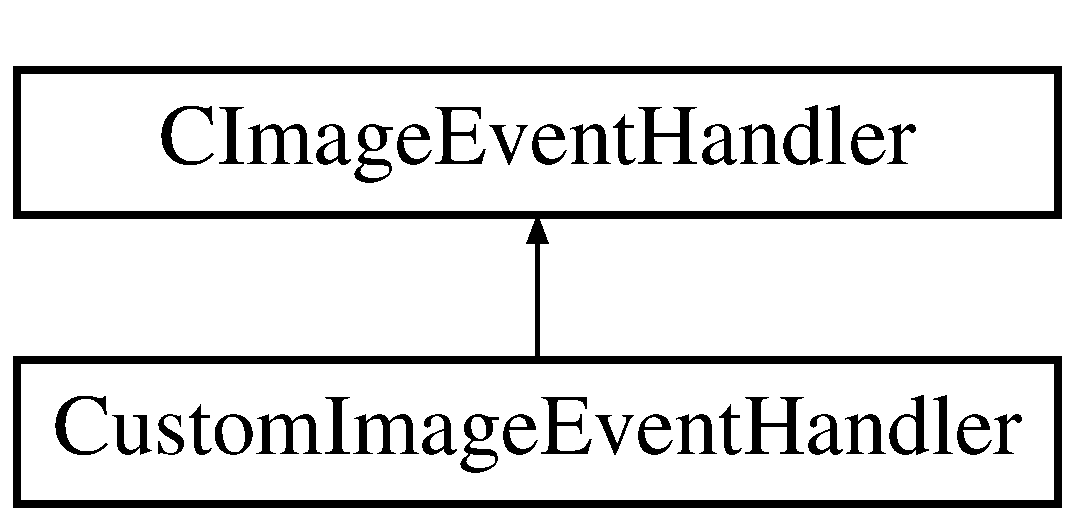
\includegraphics[height=2.000000cm]{class_custom_image_event_handler}
\end{center}
\end{figure}
\subsection*{Public Member Functions}
\begin{DoxyCompactItemize}
\item 
\mbox{\Hypertarget{class_custom_image_event_handler_aa316ec6c7965e60e0961d47c0c840b71}\label{class_custom_image_event_handler_aa316ec6c7965e60e0961d47c0c840b71}} 
{\bfseries Custom\+Image\+Event\+Handler} (int id, int rec\+\_\+frames, int curr\+\_\+height, int curr\+\_\+width, bool motion\+\_\+activation, bool many\+\_\+files=true, F\+I\+LE $\ast$file=N\+U\+LL, std\+::string wd=N\+U\+LL)
\item 
\mbox{\Hypertarget{class_custom_image_event_handler_af475f5434b7c23b2a38f55faa1c7ae6d}\label{class_custom_image_event_handler_af475f5434b7c23b2a38f55faa1c7ae6d}} 
float {\bfseries get\+Interval\+Acc} ()
\item 
\mbox{\Hypertarget{class_custom_image_event_handler_a1a0befdf9df3e4d6adcdb0db1e94341f}\label{class_custom_image_event_handler_a1a0befdf9df3e4d6adcdb0db1e94341f}} 
int {\bfseries get\+Missed\+Frames} ()
\item 
\mbox{\Hypertarget{class_custom_image_event_handler_ad6b912e16585b108301f8fed281b9ef0}\label{class_custom_image_event_handler_ad6b912e16585b108301f8fed281b9ef0}} 
int {\bfseries get\+Frame\+Number} (int i)
\item 
\mbox{\Hypertarget{class_custom_image_event_handler_a7f0ef648d61b5f108ba1181471782ffc}\label{class_custom_image_event_handler_a7f0ef648d61b5f108ba1181471782ffc}} 
int {\bfseries get\+Timestamp} (int i)
\item 
\mbox{\Hypertarget{class_custom_image_event_handler_a27ba6a6e5b1823acbc12c279eede0cce}\label{class_custom_image_event_handler_a27ba6a6e5b1823acbc12c279eede0cce}} 
virtual void {\bfseries On\+Image\+Grabbed} (C\+Instant\+Camera \&camera, const C\+Grab\+Result\+Ptr \&ptr\+\_\+grab\+\_\+result)
\end{DoxyCompactItemize}
\subsection*{Public Attributes}
\begin{DoxyCompactItemize}
\item 
\mbox{\Hypertarget{class_custom_image_event_handler_a2db3a98b441e949ff23b160a4f8b589b}\label{class_custom_image_event_handler_a2db3a98b441e949ff23b160a4f8b589b}} 
int {\bfseries recorded\+\_\+frames} = 0
\end{DoxyCompactItemize}


The documentation for this class was generated from the following file\+:\begin{DoxyCompactItemize}
\item 
/\+Users/rlaporte/\+Library/\+Mobile Documents/com$\sim$apple$\sim$\+Cloud\+Docs/\+Courses/\+B\+A\+P\+R\+O\+J -\/ Neuro-\/\+Engineering Laboratory/\+Source Files/\+N\+I\+R\+\_\+\+Imaging/\+C++\+\_\+\+Source/N\+I\+R\+\_\+\+Imaging\+\_\+\+B\+A\+S\+L\+E\+R.\+cpp\end{DoxyCompactItemize}

%--- End generated contents ---

% Index
\backmatter
\newpage
\phantomsection
\clearemptydoublepage
\addcontentsline{toc}{chapter}{Index}
\printindex

\end{document}
